
\documentclass[border=8pt, multi, tikz]{standalone} 
\usepackage{import}
\subimport{../layers/}{init}
\usetikzlibrary{positioning}
\usetikzlibrary{3d} %for including external image 

\def\ConvColor{rgb:yellow,5;red,2.5;white,5}
\def\DcnvColor{rgb:blue,5;green,2.5;white,5}
\def\ConvReluColor{rgb:yellow,5;red,5;white,5}
\def\PoolColor{rgb:red,1;black,0.3}
\def\ReluColor{rgb:red,2;blue,0.1}
\def\UnpoolColor{rgb:blue,2;green,1;black,0.3}
\def\FcColor{rgb:blue,5;red,2.5;white,5}
\def\FcReluColor{rgb:blue,5;red,5;white,4}
\def\SoftmaxColor{rgb:magenta,5;black,7}   
\def\SumColor{rgb:blue,5;green,15}

\newcommand{\copymidarrow}{\tikz \draw[-Stealth,line width=0.8mm,draw={rgb:blue,4;red,1;green,1;black,3}] (-0.3,0) -- ++(0.3,0);}

\begin{document}
\begin{tikzpicture}
\tikzstyle{connection}=[ultra thick,every node/.style={sloped,allow upside down},draw=\edgecolor,opacity=0.7]
\tikzstyle{copyconnection}=[ultra thick,every node/.style={sloped,allow upside down},draw={rgb:blue,4;red,1;green,1;black,3},opacity=0.7]

\node[canvas is zy plane at x=0] (temp) at (-2,0,0) {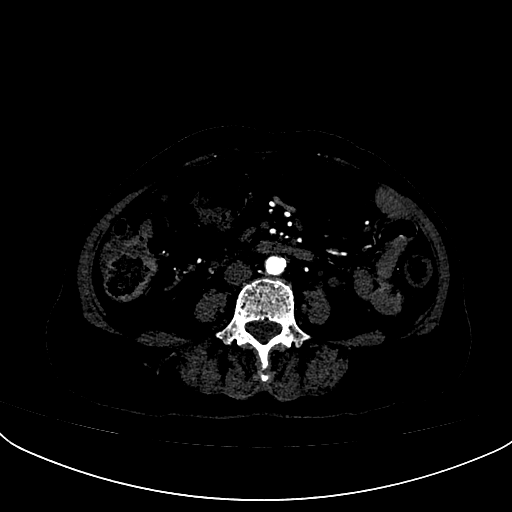
\includegraphics[width=8cm,height=8cm]{ id01_18_origin.png}};

\pic[shift={(0.5,0,0)}] at (0,0,0) 
    {Box={
        name=conv2,
        caption=DnCNN,
        xlabel={{64, }},
        zlabel=256,
        fill=\DcnvColor,
        height=35,
        width=5,
        depth=35
        }
    };

\pic[shift={ (0,0,0) }] at (conv2-east) 
    {Box={
        name=pool_conv2,
        caption= ,
        fill=\ReluColor,
        opacity=0.5,
        height=35,
        width=1,
        depth=35
        }
    };

\pic[shift={(1.5,0,0)}] at (pool_conv2-east) 
    {Box={
        name=conv3,
        caption= ,
        xlabel={{64, }},
        zlabel=256,
        fill=\DcnvColor,
        height=35,
        width=5,
        depth=35
        }
    };

\pic[shift={(0,0,0)}] at (conv3-east) 
    {Box={
        name=conv35,
        caption= ,
        xlabel={{64, }},
        zlabel=256,
        fill=\ConvColor,
        height=35,
        width=5,
        depth=35
        }
    };

\pic[shift={ (0,0,0) }] at (conv35-east) 
    {Box={
        name=pool_conv3,
        caption= ,
        fill=\ReluColor,
        opacity=0.5,
        height=35,
        width=1,
        depth=35
        }
    };

\draw [connection]  (pool_conv2-east)    -- node {\midarrow} (conv3-west);

\pic[shift={(1.5,0,0)}] at (pool_conv3-east) 
    {Box={
        name=conv4,
        caption= ,
        xlabel={{64, }},
        zlabel=256,
        fill=\DcnvColor,
        height=35,
        width=5,
        depth=35
        }
    };

\pic[shift={(0,0,0)}] at (conv4-east) 
    {Box={
        name=conv45,
        caption= ,
        xlabel={{64, }},
        zlabel=256,
        fill=\ConvColor,
        height=35,
        width=5,
        depth=35
        }
    };

\pic[shift={ (0,0,0) }] at (conv45-east) 
    {Box={
        name=pool_conv4,
        caption= ,
        fill=\ReluColor,
        opacity=0.5,
        height=35,
        width=1,
        depth=35
        }
    };

\draw [connection]  (pool_conv3-east)    -- node {\midarrow} (conv4-west);

\pic[shift={(1.5,0,0)}] at (pool_conv4-east) 
    {Box={
        name=conv5,
        caption= ,
        xlabel={{64, }},
        zlabel=256,
        fill=\DcnvColor,
        height=35,
        width=5,
        depth=35
        }
    };

\pic[shift={(0,0,0)}] at (conv5-east) 
    {Box={
        name=conv55,
        caption= ,
        xlabel={{64, }},
        zlabel=256,
        fill=\ConvColor,
        height=35,
        width=5,
        depth=35
        }
    };

\pic[shift={ (0,0,0) }] at (conv55-east) 
    {Box={
        name=pool_conv5,
        caption= ,
        fill=\ReluColor,
        opacity=0.5,
        height=35,
        width=1,
        depth=35
        }
    };

\draw [connection]  (pool_conv4-east)    -- node {\midarrow} (conv5-west);

\pic[shift={(1.5,0,0)}] at (pool_conv5-east) 
    {Box={
        name=conv6,
        caption= ,
        xlabel={{64, }},
        zlabel=256,
        fill=\DcnvColor,
        height=35,
        width=5,
        depth=35
        }
    };

\pic[shift={(0,0,0)}] at (conv6-east) 
    {Box={
        name=conv65,
        caption= ,
        xlabel={{64, }},
        zlabel=256,
        fill=\ConvColor,
        height=35,
        width=5,
        depth=35
        }
    };

\pic[shift={ (0,0,0) }] at (conv65-east) 
    {Box={
        name=pool_conv6,
        caption= ,
        fill=\ReluColor,
        opacity=0.5,
        height=35,
        width=1,
        depth=35
        }
    };

\draw [connection]  (pool_conv5-east)    -- node {\midarrow} (conv6-west);

\pic[shift={(2.55,0,0)}] at (conv6-east) 
    {Box={
        name=soft1,
        caption=Sigmoid,
        zlabel=256,
        fill=\SoftmaxColor,
        height=35,
        width=1,
        depth=35
        }
    };

\draw [connection]  (pool_conv6-east)    -- node {\midarrow} (soft1-west);

\end{tikzpicture}
\end{document}
